\chapter{Przestrzenie jednostajne i ciągłość jednostajna}
\label{ch:topog-przestrzenie-jednostajne}

\noindent\textbf{Cel rozdziału.}
Metryka pozwala porównywać odległości punktów niezależnie od miejsca,
w którym znajdują się one w przestrzeni. Sama topologia określa
jedynie lokalne otoczenia poszczególnych punktów. Struktura jednostajna
uogólnia metryczną bliskość par punktów, nie wymagając liczbowego
pomiaru odległości. Wprowadzimy topologię wyznaczoną przez taką
strukturę, ciągłość jednostajną, konstrukcje podprzestrzeni i iloczynów
oraz ciągi, sieci i filtry Cauchy'ego. Rozdział~13 będzie poświęcony
zupełności jednostajnej i uzupełnieniom.

\section{Relacje i struktury jednostajne}
\label{sec:topog-jednostajne-definicje}

\begin{definicja}[Odwracanie i składanie relacji]
\label{def:topog-jednostajne-relacje}
Niech $X$ będzie zbiorem i $E,F\subseteq X\times X$.
Definiujemy przekątną $\Delta_X=\{(x,x):x\in X\}$,
relację odwrotną $E^{-1}=\{(y,x):(x,y)\in E\}$,
przekrój $E[x]=\{y\in X:(x,y)\in E\}$ oraz złożenie
\[
 E\circ F=\{(x,z)\in X\times X:
  \exists y\in X\ ((x,y)\in E\ \land\ (y,z)\in F)\}.
\]
Relację $E$ nazywamy \emph{symetryczną}, gdy $E=E^{-1}$.
\end{definicja}

\begin{definicja}[Struktura jednostajna]
\label{def:topog-jednostajne-struktura}
\emph{Strukturą jednostajną} na zbiorze $X$ nazywamy
niepustą rodzinę $\mathcal U$ podzbiorów $X\times X$,
której elementy nazywamy \emph{otoczeniami jednostajnymi
przekątnej}, spełniającą warunki:
\begin{enumerate}[label=(\roman*)]
\item $\Delta_X\subseteq E$ dla każdego $E\in\mathcal U$;
\item jeżeli $E\in\mathcal U$ i $E\subseteq H\subseteq X\times X$,
      to $H\in\mathcal U$;
\item jeżeli $E,F\in\mathcal U$, to $E\cap F\in\mathcal U$;
\item jeżeli $E\in\mathcal U$, to $E^{-1}\in\mathcal U$;
\item dla każdego $E\in\mathcal U$ istnieje $F\in\mathcal U$
      takie, że $F\circ F\subseteq E$.
\end{enumerate}
Parę $(X,\mathcal U)$ nazywamy \emph{przestrzenią jednostajną}.
Nie wymagamy aksjomatu Hausdorffa.
\end{definicja}

\begin{uwaga}[Przestrzeń pusta]
Jeśli $X=\varnothing$, jedyną strukturą jednostajną jest
$\{\varnothing\}$. W szczególności nie wymagamy, aby każdy
element $\mathcal U$ był niepusty. Dla $X\ne\varnothing$
niepustość wynika z zawierania przekątnej.
\end{uwaga}

\begin{lemat}[Symetryczne otoczenie o małym złożeniu]
\label{lem:topog-jednostajne-symetryczne}
Dla każdego $E\in\mathcal U$ istnieje symetryczne
$F\in\mathcal U$ takie, że $F\subseteq E$ oraz
$F\circ F\subseteq E$.
\end{lemat}
\begin{proof}
Z aksjomatu (v) wybieramy $V\in\mathcal U$
z $V\circ V\subseteq E$. Kładziemy
$F=V\cap V^{-1}\cap E\cap E^{-1}$.
Z aksjomatów (iii) i (iv) wynika, że $F\in\mathcal U$;
z definicji $F=F^{-1}$ oraz $F\subseteq V\cap E$.
Wobec tego $F\circ F\subseteq V\circ V\subseteq E$.
\end{proof}

\begin{przyklad}[Dwie skrajne struktury]
\label{ex:topog-jednostajne-skrajne}
Na dowolnym zbiorze $X$ struktura
$\mathcal U_{\mathrm{ind}}=\{X\times X\}$ jest
\emph{niedyskretna}. Strukturę
$\mathcal U_{\mathrm{dysk}}=
\{E\subseteq X\times X:\Delta_X\subseteq E\}$
nazywamy \emph{dyskretną}. W drugim przypadku
aksjomat (v) spełnia $F=\Delta_X$, ponieważ
$\Delta_X\circ\Delta_X=\Delta_X$.
Obie konstrukcje działają także dla $X=\varnothing$.
\end{przyklad}

\section{Topologia wyznaczona przez strukturę jednostajną}
\label{sec:topog-jednostajne-topologia}

\begin{twierdzenie}[Topologia indukowana]
\label{thm:topog-jednostajne-topologia}
Niech $(X,\mathcal U)$ będzie przestrzenią jednostajną.
Rodzina
\[
 \tau_{\mathcal U}=
 \{O\subseteq X:\ \forall x\in O\ \exists E\in\mathcal U
                   \ (E[x]\subseteq O)\}
\]
jest topologią na $X$. Dla każdego $x\in X$
rodzina $\{E[x]:E\in\mathcal U\}$ stanowi bazę
otoczeń $x$ (niekoniecznie otwartych).
\end{twierdzenie}
\begin{proof}
Zbiór pusty spełnia podany warunek w sposób pusty.
Ponieważ $\mathcal U$ jest niepusta, dla $O=X$
można wziąć dowolne $E\in\mathcal U$.
Jeżeli $x$ należy do sumy zbiorów należących do
$\tau_{\mathcal U}$, to leży w jednym z nich i
odpowiedni przekrój $E[x]$ mieści się w całej sumie.
Jeśli $x\in O_1\cap O_2$, wybieramy
$E_i[x]\subseteq O_i$ dla $E_i\in\mathcal U$;
wtedy $(E_1\cap E_2)[x]\subseteq O_1\cap O_2$.
To dowodzi aksjomatów topologii.

Pokażemy, że każdy $E[x]$ jest otoczeniem $x$.
Niech
\[
 W=\{y\in X:\exists D\in\mathcal U\
                         (D[y]\subseteq E[x])\}.
\]
Ponieważ $E[x]\subseteq E[x]$, mamy $x\in W$,
a z $\Delta_X\subseteq D$ wynika $W\subseteq E[x]$.
Jeśli $y\in W$, wybieramy $D\in\mathcal U$
z $D[y]\subseteq E[x]$ oraz $F\in\mathcal U$
z $F\circ F\subseteq D$. Dla $z\in F[y]$ i
$w\in F[z]$ mamy $(y,w)\in F\circ F\subseteq D$,
więc $w\in E[x]$. Zatem $F[z]\subseteq E[x]$,
co oznacza $z\in W$. Dowiedliśmy $F[y]\subseteq W$,
a więc $W\in\tau_{\mathcal U}$.
Otrzymujemy $x\in W\subseteq E[x]$.

Odwrotnie, jeśli $V$ jest otoczeniem $x$,
to istnieje otwarty $O$ z $x\in O\subseteq V$.
Z definicji $\tau_{\mathcal U}$ można wybrać
$E\in\mathcal U$ z $E[x]\subseteq O\subseteq V$.
Jest to żądana własność bazy otoczeń.
\end{proof}

\begin{twierdzenie}[Kryterium Hausdorffa]
\label{thm:topog-jednostajne-hausdorff}
Dla przestrzeni jednostajnej $(X,\mathcal U)$
równoważne są warunki:
\begin{enumerate}[label=(\roman*)]
\item topologia $\tau_{\mathcal U}$ spełnia aksjomat Hausdorffa;
\item $\bigcap_{E\in\mathcal U}E=\Delta_X$.
\end{enumerate}
Strukturę spełniającą (ii) nazywamy \emph{rozdzielającą}.
\end{twierdzenie}
\begin{proof}
Jeśli topologia spełnia aksjomat Hausdorffa,
to dla $x\ne y$ istnieje otwarty $O$ z
$x\in O$ i $y\notin O$. Z definicji
topologii wybieramy $E\in\mathcal U$ z
$E[x]\subseteq O$, a zatem $(x,y)\notin E$.
Każda relacja $E\in\mathcal U$ zawiera przekątną,
stąd zachodzi (ii).

Załóżmy (ii) i ustalmy $x\ne y$. Wybieramy
$E\in\mathcal U$ z $(x,y)\notin E$ oraz
symetryczne $F\in\mathcal U$ z
$F\circ F\subseteq E$,
korzystając z lematu~\ref{lem:topog-jednostajne-symetryczne}.
Gdyby $z\in F[x]\cap F[y]$, z symetrii mielibyśmy
$(x,z),(z,y)\in F$, a więc $(x,y)\in E$,
co jest sprzecznością. Zbiory $F[x]$ i $F[y]$
są zatem rozłącznymi otoczeniami odpowiednich punktów.
Z twierdzenia~\ref{thm:topog-jednostajne-topologia}
każde zawiera otwarte otoczenie swojego punktu,
co dowodzi warunku Hausdorffa.
\end{proof}

\begin{wniosek}[Topologie skrajnych struktur]
\label{cor:topog-jednostajne-skrajne-topologie}
Topologia indukowana przez $\mathcal U_{\mathrm{ind}}$
jest niedyskretna, a przez $\mathcal U_{\mathrm{dysk}}$
dyskretna.
\end{wniosek}
\begin{proof}
W pierwszym przypadku $E[x]=X$ dla jedynej
relacji $E=X\times X$. Niepusty zbiór otwarty
musi więc być całym $X$. W drugim
$\Delta_X[x]=\{x\}$; dla każdego $O\subseteq X$
i $x\in O$ przekrój ten zawiera się w $O$.
\end{proof}

\section{Struktury wyznaczone przez metryki i pseudometryki}
\label{sec:topog-jednostajne-metryczne}

\begin{twierdzenie}[Struktura jednostajna pseudometryki]
\label{thm:topog-jednostajne-pseudometryka}
Niech $p$ będzie pseudometryką na zbiorze $X$.
Dla $\varepsilon>0$ oznaczmy
$E_\varepsilon=\{(x,y)\in X\times X:p(x,y)<\varepsilon\}$.
Wtedy
\[
 \mathcal U_p=\{E\subseteq X\times X:
      \exists\varepsilon>0\ (E_\varepsilon\subseteq E)\}
\]
jest strukturą jednostajną, a $\tau_{\mathcal U_p}$
jest topologią wyznaczoną przez $p$
w rozdziale~10. Struktura $\mathcal U_p$
jest rozdzielająca wtedy i tylko wtedy, gdy
$p$ jest metryką.
\end{twierdzenie}
\begin{proof}
Każdy $E_\varepsilon$ zawiera przekątną
i jest symetryczny. Domykanie w górę wynika
z definicji. Dla $E_\varepsilon,E_\delta$
zachodzi $E_{\min\{\varepsilon,\delta\}}
\subseteq E_\varepsilon\cap E_\delta$,
co daje domknięcie na przecięcia. Wreszcie
$E_{\varepsilon/2}\circ E_{\varepsilon/2}
\subseteq E_\varepsilon$ z nierówności trójkąta.
Jeśli $E$ zawiera $E_\varepsilon$,
możemy więc wybrać $F=E_{\varepsilon/2}$
do aksjomatu złożenia.
Dla każdego $x$ mamy
$E_\varepsilon[x]=B_p(x,\varepsilon)$.
Są to bazy otoczeń w obu topologiach,
stąd $\tau_{\mathcal U_p}=\tau_p$.
Przecięcie wszystkich $E_\varepsilon$
jest zbiorem par $(x,y)$ o $p(x,y)=0$.
Z twierdzenia~\ref{thm:topog-jednostajne-hausdorff}
otrzymujemy ostatnią równoważność.
\end{proof}

\begin{figure}[htbp]
\centering
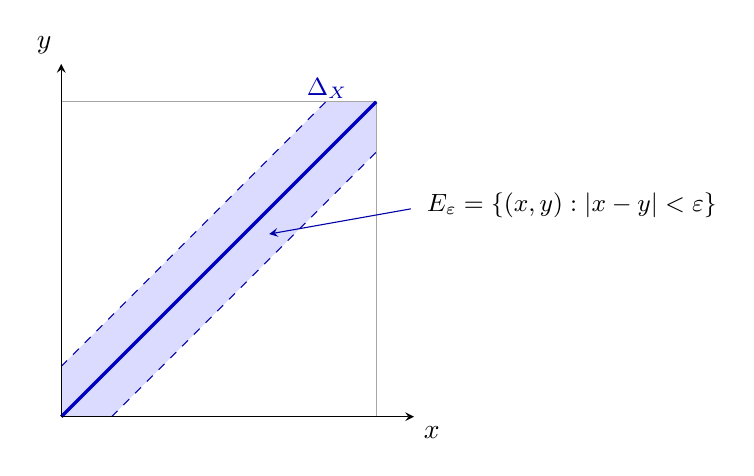
\begin{tikzpicture}[x=0.8cm,y=0.8cm,>=stealth]
\fill[blue!14] (0,0)--(.8,0)--(5,4.2)--(5,5)--(4.2,5)--(0,.8)--cycle;
\draw[gray!70] (0,0) rectangle (5,5);
\draw[very thick,blue!75!black] (0,0)--(5,5);
\draw[dashed,blue!65!black] (0,.8)--(4.2,5);
\draw[dashed,blue!65!black] (.8,0)--(5,4.2);
\draw[->] (0,0)--(5.6,0) node[below right] {$x$};
\draw[->] (0,0)--(0,5.6) node[above left] {$y$};
\node[blue!70!black,anchor=south east,font=\small] at (4.7,4.9)
 {$\Delta_X$};
\node[anchor=west,font=\small] at (5.65,3.35)
 {$E_\varepsilon=\{(x,y):|x-y|<\varepsilon\}$};
\draw[->,blue!65!black] (5.55,3.3)--(3.3,2.9);
\end{tikzpicture}
\caption{Schemat otoczenia jednostajnego przekątnej dla metryki
$|x-y|$ na przedziale $X=[0,5]$ i $\varepsilon=0{,}8$.
Zacieniowany pas zawiera przekątną. Linie przerywane
nie należą do relacji $E_\varepsilon$.}
\label{fig:topog-jednostajne-metryczny-pas}
\end{figure}

\begin{przyklad}[Ta sama topologia, różne struktury jednostajne]
\label{ex:topog-jednostajne-dwie-metryki}
Na $\R$ rozważmy metryki
$d(x,y)=|x-y|$ oraz
$e(x,y)=|\arctan x-\arctan y|$.
Ponieważ $\arctan$ jest homeomorfizmem
$\R$ na $(-\pi/2,\pi/2)$, obie metryki
wyznaczają zwykłą topologię prostej,
jak wyjaśniono w rozdziale~10.
Nie wyznaczają jednak tej samej struktury
jednostajnej. Istotnie, dla $x=n$ i $y=n+2$
mamy $d(x,y)=2$, podczas gdy
$e(n,n+2)\to0$. Dla żadnego $\delta>0$
nie zachodzi więc
$\{(x,y):e(x,y)<\delta\}
 \subseteq\{(x,y):d(x,y)<1\}$.
A zatem relacja $\{d<1\}$ należy do
$\mathcal U_d$, lecz nie do $\mathcal U_e$.
Ta różnica będzie ważna przy badaniu
zupełności w rozdziale~13.
\end{przyklad}

\section{Podprzestrzenie i iloczyny}
\label{sec:topog-jednostajne-konstrukcje}

\begin{twierdzenie}[Struktura jednostajna podprzestrzeni]
\label{thm:topog-jednostajne-podprzestrzen}
Jeśli $(X,\mathcal U)$ jest przestrzenią jednostajną,
a $A\subseteq X$, to rodzina
\[
 \mathcal U|_A=\{H\subseteq A\times A:
       \exists E\in\mathcal U\
          (E\cap(A\times A)\subseteq H)\}
\]
jest strukturą jednostajną na $A$.
Indukuje ona topologię podprzestrzeni
$(A,\tau_{\mathcal U}|_A)$.
\end{twierdzenie}
\begin{proof}
Przecięcia relacji z $A\times A$ zawierają
$\Delta_A$, zachowują odwracanie i przecięcia.
Jeśli $F\circ F\subseteq E$, to
$(F\cap(A\times A))\circ(F\cap(A\times A))
\subseteq E\cap(A\times A)$.
Daje to wszystkie aksjomaty struktury jednostajnej.

Przekroje bazowych relacji na $A$ mają postać
$(E\cap(A\times A))[a]=E[a]\cap A$.
Z twierdzenia~\ref{thm:topog-jednostajne-topologia}
są one otoczeniami $a$ w topologii względnej.
Każde względnie otwarte otoczenie $a$ ma
postać $A\cap O$, gdzie $O$ jest otwarty
w $X$; wybierając $E[a]\subseteq O$,
otrzymujemy bazowy przekrój zawarty w
$A\cap O$. Bazy otoczeń obu topologii są
więc równoważne.
\end{proof}

\begin{twierdzenie}[Produkt przestrzeni jednostajnych]
\label{thm:topog-jednostajne-iloczyn}
Niech $(X_i,\mathcal U_i)$, $i\in I$, będzie
rodziną przestrzeni jednostajnych i
$X=\prod_{i\in I}X_i$. Dla skończonego
$F\subseteq I$ oraz $E_i\in\mathcal U_i$,
$i\in F$, definiujemy
\[
 E(F,(E_i))=\{(x,y)\in X\times X:
     (x_i,y_i)\in E_i\text{ dla każdego }i\in F\}.
\]
Rodzina wszystkich nadzbiorów tych relacji
jest strukturą jednostajną $\mathcal U_\Pi$.
Jej topologia jest topologią iloczynu topologii
$\tau_{\mathcal U_i}$. Każde rzutowanie
$\pi_i:X\to X_i$ jest jednostajnie ciągłe
w sensie definicji podanej w następnej sekcji.
\end{twierdzenie}
\begin{proof}
Każda bazowa relacja zawiera przekątną.
Dla dwóch relacji bazowych warunek z
ich przecięcia uzyskujemy na sumie skończonych
zbiorów współrzędnych, biorąc przecięcie
odpowiednich relacji tam, gdzie indeksy się
powtarzają. Odwracanie wykonujemy
współrzędna po współrzędnej. Do warunku
złożenia wybieramy dla każdego $i\in F$
relację $H_i$ z $H_i\circ H_i\subseteq E_i$;
wówczas
$E(F,(H_i))\circ E(F,(H_i))
\subseteq E(F,(E_i))$.
Aksjomaty domykania w górę są zawarte
w samej definicji $\mathcal U_\Pi$.

Ustalmy $x\in X$. Przekroje bazowych relacji
mają postać
$\bigcap_{i\in F}\pi_i^{-1}(E_i[x_i])$.
Na mocy twierdzenia~\ref{thm:topog-jednostajne-topologia}
każdy $E_i[x_i]$ jest otoczeniem $x_i$;
zatem taki przekrój jest otoczeniem
$x$ w topologii iloczynu. Odwrotnie,
dla każdego bazowego otwartego cylindra
$\bigcap_{i\in F}\pi_i^{-1}(O_i)$
zawierającego $x$ istnieją
$E_i\in\mathcal U_i$ z $E_i[x_i]\subseteq O_i$.
Odpowiedni przekrój $E(F,(E_i))[x]$
mieści się w cylindrze. Obie topologie
mają więc takie same otoczenia.

Ostatnie twierdzenie wynika wprost z tego,
że dla dowolnego $E_i\in\mathcal U_i$
relacja $E(\{i\},(E_i))$ należy do
$\mathcal U_\Pi$ i jej pary mają
$i$-te współrzędne należące do $E_i$.
\end{proof}

\begin{uwaga}[Produkt pustej rodziny]
Dla $I=\varnothing$ iloczyn zbiorów
jest przestrzenią jednoelementową,
a jedyną bazową relacją w konstrukcji
jest $X\times X=\Delta_X$.
Jeśli któryś czynnik jest pusty,
cały iloczyn jest pusty i otrzymujemy
jedyną strukturę jednostajną na zbiorze pustym.
\end{uwaga}

\section{Odwzorowania jednostajnie ciągłe}
\label{sec:topog-jednostajne-ciaglosc}

\begin{definicja}[Ciągłość jednostajna]
\label{def:topog-jednostajne-ciaglosc}
Niech $(X,\mathcal U)$ i $(Y,\mathcal V)$
będą przestrzeniami jednostajnymi.
Odwzorowanie $f:X\to Y$ jest
\emph{jednostajnie ciągłe}, jeżeli
dla każdego $V\in\mathcal V$ istnieje
$E\in\mathcal U$ takie, że
$(x,x')\in E$ pociąga za sobą
$(f(x),f(x'))\in V$ dla wszystkich $x,x'\in X$.
Dla struktur metrycznych odpowiada to
zwykłemu warunkowi $\varepsilon$--$\delta$,
w którym $\delta$ nie zależy od punktu $x$.
\end{definicja}

\begin{twierdzenie}[Ciągłość i składanie]
\label{thm:topog-jednostajne-ciaglosc-wlasnosci}
Niech $X,Y,Z$ będą przestrzeniami jednostajnymi.
Każde odwzorowanie jednostajnie ciągłe
$f:X\to Y$ jest ciągłe w topologiach
indukowanych. Jeśli ponadto
$g:Y\to Z$ jest jednostajnie ciągłe,
to $g\circ f:X\to Z$ jest jednostajnie ciągłe.
\end{twierdzenie}
\begin{proof}
Ustalmy $x\in X$ oraz otwarte otoczenie
$O$ punktu $f(x)$ w $Y$. Istnieje
$V\in\mathcal V$ z $V[f(x)]\subseteq O$.
Wybieramy $E\in\mathcal U$ na mocy
ciągłości jednostajnej. Wówczas
$f(E[x])\subseteq V[f(x)]\subseteq O$.
Ponieważ $E[x]$ jest otoczeniem $x$,
ciągłość $f$ w punkcie $x$ wynika z
kryterium otoczeń.

Dla $W$ należącego do struktury na $Z$
wybieramy $V$ na $Y$, które $g$ przenosi
w $W$, a następnie $E$ na $X$, które
$f$ przenosi w $V$. Dla $(x,x')\in E$
para $(g(f(x)),g(f(x')))$ należy do $W$,
co jest dokładnie definicją.
\end{proof}

\begin{przyklad}[Odwzorowanie ciągłe, ale nie jednostajnie ciągłe]
\label{ex:topog-jednostajne-kwadrat}
Funkcja $f:\R\to\R$, $f(x)=x^2$, jest
ciągła w zwykłej topologii.
Nie jest jednostajnie ciągła dla
struktur wyznaczonych metryką euklidesową.
Rzeczywiście, weźmy $x_n=n$ i
$y_n=n+1/n$. Wtedy $|x_n-y_n|=1/n\to0$,
lecz $|f(y_n)-f(x_n)|=2+1/n^2\ge2$.
Dla $\varepsilon=1$ żadne $\delta>0$
nie spełnia warunku ciągłości jednostajnej.
\end{przyklad}

\begin{lemat}[Zwartość metryczna implikuje zwartość ciągową]
\label{lem:topog-jednostajne-zwarta-ciagowa}
Niech $(K,d)$ będzie zwartą przestrzenią metryczną.
Wówczas każdy ciąg $(x_n)_{n\ge1}$ w $K$ ma
podciąg zbieżny do pewnego punktu $x\in K$.
\end{lemat}
\begin{proof}
Dla każdego $N\ge1$ niech
$F_N=\overline{\{x_n:n\ge N\}}^{\,K}$.
Są to niepuste zbiory domknięte w $K$,
a ponadto $F_{N+1}\subseteq F_N$.
Każda skończona rodzina tych zbiorów ma
przecięcie równe jej najmniejszemu
elementowi w sensie inkluzji, a więc
niepuste. Z kryterium skończonych przecięć
dla zwartości, udowodnionego w
twierdzeniu~\ref{thm:topog-zwartosc-fip},
istnieje $x\in\bigcap_{N\ge1}F_N$.

Konstruujemy ściśle rosnący ciąg indeksów.
Przyjmijmy $n_0=0$. Jeśli wybrano
$n_{k-1}$, to $x\in F_{n_{k-1}+1}$.
Z definicji domknięcia punkt $x$
należy do domknięcia ogona
$\{x_n:n\ge n_{k-1}+1\}$, zatem kula
$B_d(x,1/k)$ zawiera pewien wyraz
$x_{n_k}$ tego ogona. Wybieramy
$n_k\ge n_{k-1}+1$ tak, aby
$d(x_{n_k},x)<1/k$. W rezultacie
$n_k>n_{k-1}$ i $x_{n_k}\to x$.
\end{proof}

\begin{twierdzenie}[Twierdzenie Heinego--Cantora]
\label{thm:topog-jednostajne-heine-cantor}
Niech $(K,d)$ będzie zwartą przestrzenią
metryczną, a $(Y,e)$ przestrzenią metryczną.
Każde ciągłe odwzorowanie $f:K\to Y$
jest jednostajnie ciągłe.
\end{twierdzenie}
\begin{proof}
Przypuśćmy przeciwnie, że istnieje
$\varepsilon_0>0$ takie, że dla każdego
$n\ge1$ można wybrać $x_n,y_n\in K$
z $d(x_n,y_n)<1/n$ oraz
$e(f(x_n),f(y_n))\ge\varepsilon_0$.
Na mocy lematu~\ref{lem:topog-jednostajne-zwarta-ciagowa}
ciąg $(x_n)$ ma podciąg $(x_{n_k})$
zbieżny do $x\in K$.
Z nierówności
$d(y_{n_k},x)\le d(y_{n_k},x_{n_k})
  +d(x_{n_k},x)$
wynika, że również $y_{n_k}\to x$.
Ciągłość $f$ w $x$ daje
$f(x_{n_k})\to f(x)$ i $f(y_{n_k})\to f(x)$.
Nierówność trójkąta w $Y$ prowadzi do
$e(f(x_{n_k}),f(y_{n_k}))\to0$,
wbrew wyborowi $\varepsilon_0$.
\end{proof}

\section{Ciągi, sieci i filtry Cauchy'ego}
\label{sec:topog-jednostajne-cauchy}

\begin{definicja}[Sieć Cauchy'ego]
\label{def:topog-jednostajne-siec-cauchyego}
Niech $(X,\mathcal U)$ będzie przestrzenią
jednostajną, a $D$ niepustym zbiorem skierowanym.
Sieć $(x_\alpha)_{\alpha\in D}$ jest
\emph{siecią Cauchy'ego}, jeśli dla każdego
$E\in\mathcal U$ istnieje $\alpha_0\in D$
takie, że $(x_\alpha,x_\beta)\in E$
dla wszystkich $\alpha,\beta\ge\alpha_0$.
Jeśli $D=\mathbb N$, mówimy o \emph{ciągu Cauchy'ego}.
\end{definicja}

\begin{definicja}[Filtr Cauchy'ego]
\label{def:topog-jednostajne-filtr-cauchyego}
Filtr $\mathcal F$ na $X$ nazywamy
\emph{filtrem Cauchy'ego}, jeżeli
dla każdego $E\in\mathcal U$ istnieje
$A\in\mathcal F$ takie, że $A\times A\subseteq E$.
\end{definicja}

\begin{twierdzenie}[Sieć i filtr ogonów]
\label{thm:topog-jednostajne-ogony}
Niech $(x_\alpha)_{\alpha\in D}$ będzie
siecią w przestrzeni jednostajnej $(X,\mathcal U)$.
Niech $\mathcal F_x$ będzie filtrem
generowanym przez zbiory ogonowe
$A_{\alpha_0}=\{x_\alpha:\alpha\ge\alpha_0\}$.
Wtedy sieć jest Cauchy'ego wtedy i tylko wtedy,
gdy $\mathcal F_x$ jest filtrem Cauchy'ego.
\end{twierdzenie}
\begin{proof}
Zbiory $A_{\alpha_0}$ są niepuste.
Skierowanie $D$ zapewnia, że dwa ogony
zawierają wspólny mniejszy ogon;
tworzą więc bazę filtra.
Jeśli sieć jest Cauchy'ego, dla każdego
$E\in\mathcal U$ pewien ogon spełnia
$A_{\alpha_0}\times A_{\alpha_0}\subseteq E$.
Jest on elementem $\mathcal F_x$.

Odwrotnie, niech dla $E\in\mathcal U$
istnieje $A\in\mathcal F_x$ z
$A\times A\subseteq E$. Z definicji
filtra generowanego przez ogony istnieje
$\alpha_0$ takie, że $A_{\alpha_0}\subseteq A$.
Zatem dla $\alpha,\beta\ge\alpha_0$
para $(x_\alpha,x_\beta)$ należy do $E$.
\end{proof}

\begin{twierdzenie}[Zbieżność implikuje warunek Cauchy'ego]
\label{thm:topog-jednostajne-zbiezna-cauchy}
W każdej przestrzeni jednostajnej
każda sieć zbieżna w topologii
$\tau_{\mathcal U}$ jest siecią Cauchy'ego.
\end{twierdzenie}
\begin{proof}
Załóżmy $x_\alpha\to x$. Ustalmy
$E\in\mathcal U$. Na mocy
lematu~\ref{lem:topog-jednostajne-symetryczne}
istnieje symetryczne $F\in\mathcal U$
z $F\circ F\subseteq E$.
Z twierdzenia~\ref{thm:topog-jednostajne-topologia}
zbiór $F[x]$ jest otoczeniem $x$,
więc dla wszystkich $\alpha\ge\alpha_0$
mamy $x_\alpha\in F[x]$.
Jeśli $\alpha,\beta\ge\alpha_0$, to
$(x_\alpha,x),(x,x_\beta)\in F$
dzięki symetrii. Stąd
$(x_\alpha,x_\beta)\in F\circ F\subseteq E$.
\end{proof}

\begin{stwierdzenie}[Ciągłość jednostajna zachowuje sieci Cauchy'ego]
\label{prop:topog-jednostajne-f-cauchy}
Jeżeli $f:(X,\mathcal U)\to(Y,\mathcal V)$
jest jednostajnie ciągłe, a
$(x_\alpha)$ jest siecią Cauchy'ego w $X$,
to $(f(x_\alpha))$ jest siecią Cauchy'ego w $Y$.
\end{stwierdzenie}
\begin{proof}
Dla $V\in\mathcal V$ wybieramy
$E\in\mathcal U$ takie, że
$(f\times f)(E)\subseteq V$.
Od pewnego indeksu wszystkie pary
$(x_\alpha,x_\beta)$ należą do $E$;
ich obrazy należą więc do $V$.
\end{proof}

\begin{twierdzenie}[Sieci Cauchy'ego w produkcie]
\label{thm:topog-jednostajne-produkt-cauchy}
Niech $X=\prod_{i\in I}X_i$ ma strukturę
jednostajną produktu z
twierdzenia~\ref{thm:topog-jednostajne-iloczyn}.
Sieć $(x_\alpha)$ w $X$ jest Cauchy'ego
wtedy i tylko wtedy, gdy dla każdego $i\in I$
sieć współrzędnych $(\pi_i(x_\alpha))$
jest Cauchy'ego w $X_i$.
\end{twierdzenie}
\begin{proof}
Jeśli $(x_\alpha)$ jest Cauchy'ego,
rzutowania są jednostajnie ciągłe,
więc ich sieci obrazów są Cauchy'ego
na mocy poprzedniego stwierdzenia.
Odwrotnie, ustalmy bazowe otoczenie
$E(F,(E_i))$ produktu, gdzie $F$ jest
skończony. Dla każdego $i\in F$ istnieje
indeks $\alpha_i$, od którego wszystkie
pary odpowiednich współrzędnych leżą
w $E_i$. Skierowanie zbioru indeksów
pozwala znaleźć wspólną górną granicę
skończonej rodziny $(\alpha_i)_{i\in F}$.
Od tego indeksu wszystkie pary
$(x_\alpha,x_\beta)$ należą do
$E(F,(E_i))$. Gdy $F=\varnothing$,
warunek jest automatycznie spełniony.
Każda relacja produktu zawiera bazową,
co kończy dowód.
\end{proof}

\section{Kontrprzykłady i rozróżnienia}
\label{sec:topog-jednostajne-kontrprzyklady}

\begin{przyklad}[Sieć Cauchy'ego bez granicy]
\label{ex:topog-jednostajne-cauchy-bez-granicy}
Ciąg $x_n=1/(n+1)$ w $(0,1)$ ze
strukturą indukowaną przez metrykę
euklidesową jest Cauchy'ego, gdyż
jest Cauchy'ego w $\R$. Nie ma jednak
granicy w $(0,1)$: jedyną granicą
w $\R$ jest $0$. Zatem odwrotność
twierdzenia~\ref{thm:topog-jednostajne-zbiezna-cauchy}
jest fałszywa.
\end{przyklad}

\begin{przyklad}[Zbieżność bez jednoznacznej granicy]
\label{ex:topog-jednostajne-niehausdorff}
Jeśli $X$ ma co najmniej dwa punkty
i strukturę niedyskretną, każda sieć
w $X$ zbiega do każdego punktu.
Istotnie, jedynymi otwartymi zbiorami
są $\varnothing$ i $X$. Każda sieć
jest również Cauchy'ego, ponieważ
jedyną relacją jednostajną jest $X\times X$.
Nie można zatem oczekiwać jednoznaczności
granicy bez założeń oddzielania.
\end{przyklad}

\begin{przyklad}[Topologia nie określa ciągów Cauchy'ego]
\label{ex:topog-jednostajne-cauchy-dwie-metryki}
W przykładzie~\ref{ex:topog-jednostajne-dwie-metryki}
metryki $d$ i $e$ mają tę samą topologię na $\R$,
lecz ciąg $x_n=n$ jest Cauchy'ego dla $e$,
ponieważ ciąg $\arctan(n)$ zbiega w $\R$.
Nie jest Cauchy'ego dla $d$, gdyż
$d(n,2n)=n$ dla $n\ge1$. Nie ma również
granicy w zwykłej topologii $\R$.
Zbieżność jest więc pojęciem topologicznym,
ale warunek Cauchy'ego zależy od struktury
jednostajnej.
\end{przyklad}

\begin{uwaga}[Przejście do rozdziału następnego]
W przestrzeniach jednostajnych zupełność
będziemy formułować za pomocą filtrów
lub sieci Cauchy'ego. Rozdział~13
wyjaśni, jak te pojęcia wiążą się
z zupełnością metryczną z rozdziału~11,
i skonstruuje uzupełnienia.
\end{uwaga}
